\subsection{Data Sources, Modeling choices}

We use the AME model on the two aforementioned measures of state amity to generate a combined measure of state preference similarity which accounts for network effects. We use the distance between states' ideal points (as calculated by \citet{voeten:XXXX} using UN data) and S-score for two states alliance portfolios. However, to facilitate comparison between the metrics, we first transform the S-score into a measure of distance between alliance portfolios.\footnote{D = 1 - S} We then standardize and normalize these two measures. This gives us an N by N by Y by 2 array, where the first two dimensions represent countries, the third dimension is the year, and the fourth is the particular measure of similarity. So the item at index (1,2,1,1) would be the transformed value of the S-score for countries XXX and YYY at the first year of our data (YYYY), similarly (1,2,1,2) would be the UN ideal point distance.

Another important question is the amount of temporal aggregation used. In our baseline model, we treat each year as separate and gain a unique observation of each states ideal point in each year. However, this raises a real risk of temporal inconsistency in the values. An alternative approach would be to have a rolling average for the measures of similarity over a number of years. This would allow us to infer a country's relative position not just by their behavior in a given year, but also their behavior in the past few years. The risk if we use too much temporal aggregation is that we are including data which is no longer relevant to a country's relative preferences. For instance, Turkey and Russia's relationship looks a lot more positive when we look at 2013 and 2014 then when we look at 2015. To that end, in addition to our baseline model where years are seen as independent, we also evaluate models where ... 

With this data, we run an AME model with a Gaussian link, and in particular we use the uDv term to estimate each states position in a two-dimensional latent space. We then evaluate whether their is additional utility gained from using this latent position, as compared to the component measures of similarity of alliance portfolio and UN ideal point distance.

\section{Constructing Latent Angle Measure}

\begin{figure}[ht]
	\centering
	\includegraphics[width=.7\textwidth]{latPlot}
	\caption{Latent factor plot.}
	\label{fig:latPlot}
\end{figure}

\subsection{Face Plausibility}

Are states close to who we'd expect them to be?

\subsection{Temporal Reliability}

Are our measures consistent?

\section{Model Competition}
To evaluate different measures of state preferences, we compare them in a model of interstate disputes. Here we look at four non-nested models: a model using no measures of state preferences, one using an S-Score based on similarity in alliance portfolio (as in \ref{signorino:ritter:year}, one using the ideal points determined by UN voting (as in \ref{bailey:strezhnev:voeten:year}), a model using both UN ideal points and alliance S-scores, and finally, a model using our latent angle approach to combine data from UN voting and alliances. We evaluate the models on two criteria: whether state preferences have a consistent effect in the predicted direction, and how well each model does at predicting disputes on out of sample data.

\subsection{Data, Controls}
In each of these models, we look at a logistic regression of Militarized Interstate Dispute participation on measures of state preferences and a vector of control variables. These control variables are most of the standard ones used most famously in O'Neal and Russett's work on the democratic peace \citep{oneal:russett:year}.\footnote{The exception is that our models ignore trade interdependency, as including that data drastically decreases the number of observations.} In particular, we include a binary measure of joint democracy (whether both states have Polity IV scores $geq 7$), whether the states are contiguous, and the ratio of state capabilities as measured by the Correlates of War Project's Composite Index of National Capabilities (CINC). We also account for temporal interdependence using a peace year spline, as in \ref{beck:katz:year}. 

\subsection{In sample explanation}
As detailed in figure \ref{fig:coefP}, each measure of state preferences performs as we would expect them to. Our measure of state preference using latent angle difference is highly significant and positive: states with more dissimilar preferences will have greater difference in their latent angles, and this is highly associated with a greater risk of conflict. Similarly, both incumbent measures of preferences pass this test. The measure using UN voting ideal points is positive and clearly distinct from $0$, indicating that states with more distant ideal points, and thus more dissimilar preferences, are more likely to find themselves in conflict. Similarly, higher alliance S-scores are consistently associated with lower probabilities of conflict -- so states with more similar preferences as measured using alliance portfolios are less likely to quarrel. These results hold when the measure of preferences is used in isolation, or in tandem.

The models have one major difference in terms of the controls: in the model using latent angle distance, joint democracy is indistinguishable from $0$. This is particularly interesting because of one of the major criticisms of democratic peace theory is that, for one reason or another, democracies have similar preferences, and this is what actually causes peace among democracies.  Despite this dispute, most attempts to include preferences in the standard democratic peace regressions still found a consistent pacifying effect of democracy.
(as do those models with UN voting and S-scores presented here). With our measure of preferences, however, democracy's effect is negligible.


\begin{figure}[ht]
	\centering
	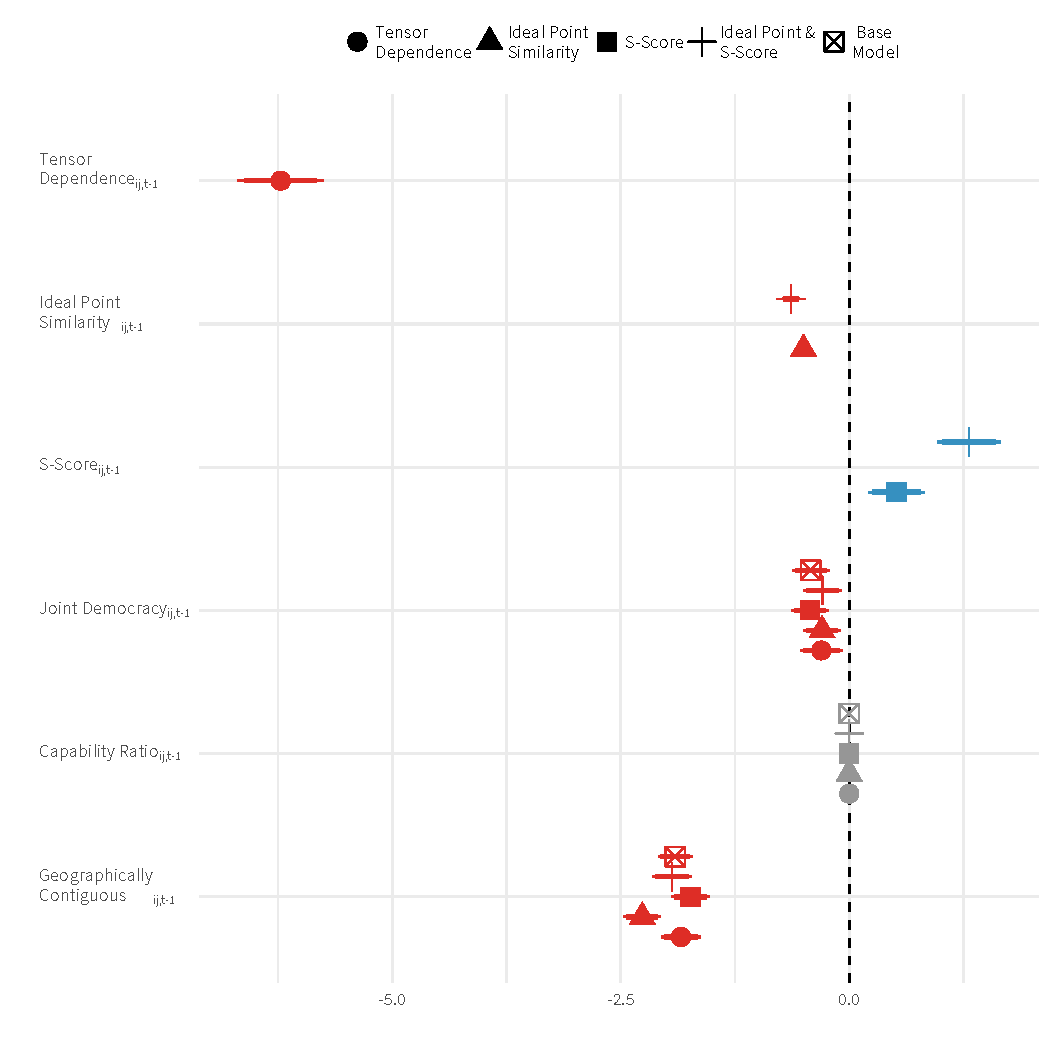
\includegraphics[width=.7\textwidth]{betaEst}
	\caption{Parameter estimates from models with different measures of state preference. Point represents average estimate, line through the point represents the 95\% confidence interval.}
	\label{fig:coefP}
\end{figure}
\FloatBarrier

\subsection{Out of sample prediction}
Given these results, we can say that all of the measures of preferences behave as we would expect. To adjudicate which measures best capture state preferences, and what we should make of the differing effect of democracy, we turn to out of sample prediction. The way we do this is by partitioning our data into 30 different folds, and for each fold we generate a predicted value for each case the other 29 folds for each model. This leaves us with a set of predicted values generated entirely out of sample. We then compare the models performance using the area under both the Receiver Operator Characteristic Curve (AUC ROC) which examines the tradeoffs between true positives and false positives, and the area under the Precision Recall Curve (AUC PR) which looks at the tradeoffs between making only correct predictions, and predicting all the disputes which occurred. In general, the AUC ROC will disproportionately reward those models that predict $0$ well, and we can interpret the AUC ROC as the likelihood a prediction is correct, the numeric value for the AUC PR has less of a clear interpretation, but models with a higher AUC PR do a better job of predicting when events actually occur.

As shown in figure \ref{fig:roc}, the model using latent angle distance decisively outperforms all the other models. While the AUC ROC is somewhat higher with the Latent Angle model, the real difference between the measures shines through in the AUC PR, where the model using this measure performs twice as well as the base model. In contrast, models using other measures of state preferences yield only minimal improvements in prediction over the base model. Thus we have real reason for confidence in both the usefulness of this measure of state preferences and renewed reason for skepticism in the effect of joint democracy once we control for state preferences. 

\begin{figure}[ht]
	\centering
	\begin{tabular}{cc}
	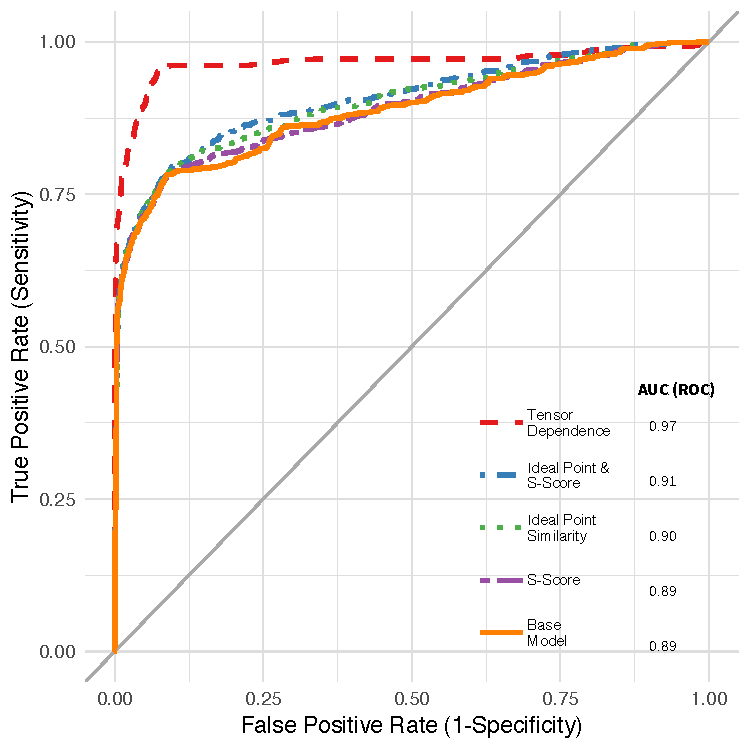
\includegraphics[width=.5\textwidth]{roc_outSample} & 
	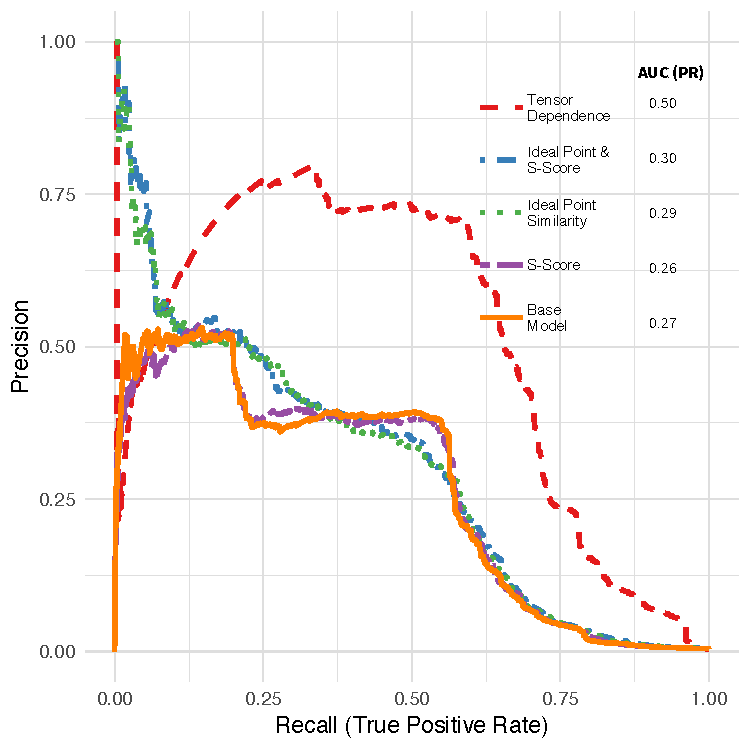
\includegraphics[width=.5\textwidth]{rocPr_outSample}	
	\end{tabular}
	\caption{Assessments of out-of-sample predictive performance using ROC curves and PR curves. AUC statistics are provided as well for both curves.}
	\label{fig:roc}
\end{figure}
\FloatBarrier

